\section{Method}
\label{sec:method}

This is method. And the figure \ref{fig:banana} shows the banana.

\begin{figure}
    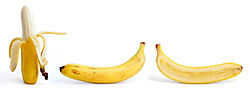
\includegraphics[width=\textwidth]{figures/banana.jpg}
    \caption{Banana}
    \label{fig:banana}
\end{figure}


- select sample of urban areas (FUA)
- fetch the data from OSM
- polygonize the network
- measure shape charactersitics
    - TODO: measure initally more than Reock (get a sample from ESDA)
    - there is a conceptual backbone to this - we know that the artifacts are either
    small (small intersections) polygons or can be large but then they are very narrow
    (in between dual carriegaway)
    - we need a shape metric that captures this relationship
- identify optimal measurements
    - plots that help us visually detect a cluster of artifacts
- derivation of 1-dimensional index
    - from Roeck and area we can derive one value from which distribution we can
    identify a cut-off value for artifact/non-artifact polygons
- cut-off value detection
- exploration of geographical variation
    - differences between cities and continents
- open tools, open data, open code with full reproducibility